% Asal-usul (tidak pernah dicetak): lihat sources/outline_sources.md (Tahun 1: pemadatan dan sementasi; jenis cekungan; penurunan, akomodasi dan perubahan muka laut). Nilai soal latihan dan soal dalam kalkulator skrap Buku 3 calc/ch23.py; data gambar dari figdata/bachelor-1/compaction.py dan sea_level.py. Porositas dan permeabilitas milik Buku 1 (kelas 6); diagenesis telah dijumpai di Buku 2 (kelas 12) dan didirikan ulang di sini; cekungan sedimen telah dijumpai di Buku 2 (kelas 11) dan didirikan ulang di sini; isostasi dan proposisi massa sama milik bab 11; margin pasif dan celah milik bab 13; tegangan efektif milik bab 16; Maksimum Glasial Terakhir dan siklus glasial milik Buku 2 (kelas 12). Sesar tekanan didefinisikan dalam volume Tahun ke-3 (mekanisme deformasi): hanya prosa. Penelusuran mundur (backstripping), model peregangan dan perbandingan cekungan milik volume Tahun ke-2.
\chapter{Diagenesis dan cekungan sedimen}\label{ch:b1:diagenesis-basins}

Pasir pantai itu lepas: separuhnya, menurut volume, adalah air di antara butiran. Terkubur tiga kilometer di bawah, pasir yang sama muncul kembali dalam inti bor sebagai batu pasir yang keras, butirannya terdesak bersama dan ruang di antaranya sangat berkurang serta sebagian terisi kuarsa baru. Di antara pantai dan inti itu terbentang jutaan tahun ketika sedimen tertimbun di bawah sedimen lain, terperas, terpanaskan dan tersiram air yang melarutkan sebagian \omterm{def:b1:rock-forming-minerals:mineral}{mineral} dan mengendapkan yang lain. Bab ini mengikuti perubahan-perubahan itu, lalu melangkah mundur ke tempat-tempat di mana sedimen dapat menumpuk setebal kilometer --- \omterm{def:b1:diagenesis-basins:basin}{cekungan sedimen} --- dan ke dua hal yang menciptakan ruang baginya di sana: \omterm{def:b1:diagenesis-basins:subsidence}{penurunan} dasar, dan naik turunnya laut.

\begin{recall}
Porositas batuan adalah fraksi volumenya yang terdiri dari pori, dan permeabilitasnya mengukur seberapa mudah air mengalir melaluinya (Buku~1, kelas~6). Suatu wilayah berada dalam \omterm{def:b1:isostasy-gravity:isostasy}{isostasi} ketika setiap kolom hingga \omterm{def:b1:isostasy-gravity:isostasy}{kedalaman kompensasi} memiliki massa yang sama (\cref{prop:b1:isostasy-gravity:equal-mass}). Celah terbuka oleh \omterm{def:b1:faults-folds-fabrics:fault-types}{sesar normal}, dan margin pasif adalah tepi benua yang tertinggal ketika sebuah celah menjadi samudra (\cref{ch:b1:rifts-ridges-margins}). \omterm{def:b1:stress-strain-rheology:lithostatic}{Tegangan efektif} adalah tegangan dikurangi \omterm{def:b1:stress-strain-rheology:lithostatic}{tekanan fluida pori} (\cref{def:b1:stress-strain-rheology:lithostatic}). Siklus glasial terakhir mencapai Maksimum Glasial Terakhir sekitar dua puluh ribu tahun yang lalu (Buku~2, kelas~12). Batu pasir, serpih dan lingkungannya adalah yang ada dalam \cref{ch:b1:clastic-sediments}; batu kapur, kapur, dolomit dan \omterm{def:b1:chemical-biogenic-sediments:evaporite}{evaporit} adalah yang ada dalam \cref{ch:b1:chemical-biogenic-sediments}.
\end{recall}

\section{Pemadatan}\label{sec:b1:diagenesis-basins:compaction}

Sedimen yang baru diendapkan adalah tumpukan butiran lepas dengan air di antaranya. Segala yang terjadi padanya setelah pengendapan dan sebelum metamorfisme, selagi ia tetap berada pada suhu dan tekanan rendah dari beberapa kilometer atas \omterm{def:b1:layered-earth:layers}{kerak}, termasuk dalam satu keluarga proses.

\begin{definition}[Diagenesis sedimen]\label{def:b1:diagenesis-basins:diagenesis}
\emph{Diagenesis}\index{diagenesis} adalah himpunan perubahan fisika, kimia dan biologi yang dialami sedimen setelah pengendapannya, pada suhu dan tekanan \omterm{def:b1:layered-earth:layers}{kerak} atas, di bawah yang dimiliki metamorfisme. Ia mencakup \omterm{def:b1:diagenesis-basins:compaction}{pemadatan}, \omterm{def:b1:diagenesis-basins:cement}{sementasi}, pelarutan butiran, dan penggantian satu \omterm{def:b1:rock-forming-minerals:mineral}{mineral} oleh \omterm{def:b1:rock-forming-minerals:mineral}{mineral} lain; bersama-sama mereka mengubah sedimen lepas menjadi batuan sedimen.
\end{definition}

Perubahan pertama bersifat mekanis. Setiap lapisan baru menambahkan beratnya pada lapisan di bawahnya. Butiran-butiran terdesak bersama, bergeser dan berputar menjadi susunan yang lebih rapat, yang lunak (serpihan lempung, fragmen batuan, \omterm{def:b1:rock-forming-minerals:groups}{mika}) melentur di antara yang keras, dan air di antara mereka terperas keluar.
% ledger: og:diagenesis

\begin{definition}[Pemadatan, dekompaksi]\label{def:b1:diagenesis-basins:compaction}
\emph{Pemadatan}\index{pemadatan} adalah hilangnya volume sedimen di bawah berat sedimen di atasnya, akibat susunan butirannya yang lebih rapat, keluarnya air porinya dan, lebih dalam, pelarutan butiran di tempat mereka bersentuhan. \emph{Dekompaksi}\index{dekompaksi} adalah perhitungan yang memulihkan lapisan terkubur ke ketebalan yang dimilikinya pada penguburan yang lebih awal dan lebih dangkal, paling sering di permukaan, ketika ia diendapkan.
\end{definition}

Porositas yang diukur di sumur turun seiring kedalaman, curam di dekat permukaan dan kemudian makin lama makin lambat. Pada 1930 L.~F. Athy mencocokkannya dengan eksponensial, dan kecocokan itu telah menjadi titik awal studi \omterm{def:b1:diagenesis-basins:compaction}{pemadatan} sejak saat itu.
% ledger: sc80:athy

\begin{proposition}[Hukum Athy]\label{prop:b1:diagenesis-basins:athy}
Dalam tumpukan sedimen dari satu litologi, yang dipadatkan oleh beratnya sendiri dengan air porinya bebas keluar, porositas pada kedalaman $z$ di bawah permukaan adalah
\[
  \varphi(z) = \varphi_0\, e^{-z/\lambda},
\]
di mana $\varphi_0$, porositas permukaan, dan $\lambda$, panjang peluruhan, bergantung pada litologi. Inilah \emph{hukum Athy}\index{hukum Athy}.
\end{proposition}
\admitted

Hukum ini adalah kecocokan empiris, bukan konsekuensi teori. Parameternya diukur, litologi demi litologi, dari porositas sumur; nilai-nilai dalam \cref{tab:b1:diagenesis-basins:athy}, yang diterbitkan bersama studi \omterm{def:b1:diagenesis-basins:subsidence}{penurunan} Laut Utara, banyak dipakai untuk mengoreksi \omterm{def:b1:diagenesis-basins:compaction}{pemadatan}. Serpih mulai dengan lebih banyak air daripada pasir tetapi kehilangannya dalam jarak yang lebih pendek; kapur, yang paling berpori dari ketiganya di permukaan, kehilangannya paling cepat dari semuanya. Pada \qty{3000}{m} hukum itu memberi porositas \num{0.22} untuk batu pasir, \num{0.14} untuk serpih dan \num{0.08} untuk kapur (gambar di bawah): pasir pantai di awal bab telah kehilangan lebih dari separuh porinya.
% ledger: pybacktrack:compaction, sc80:north-sea

\begin{table}[htbp]
\centering
\begin{tabular}{lccc}
\hline
litologi & \shortstack{porositas\\permukaan $\varphi_0$} & \shortstack{panjang\\peluruhan $\lambda$ (m)} & \shortstack{massa jenis\\butiran (\unit{kg.m^{-3}})} \\
\hline
serpih            & 0.63 & 1960 & 2700 \\
batu pasir        & 0.49 & 3704 & 2650 \\
batu pasir lempungan  & 0.56 & 2564 & 2680 \\
kapur            & 0.70 & 1408 & 2710 \\
\hline
\end{tabular}
\caption{Parameter \omterm{prop:b1:diagenesis-basins:athy}{hukum Athy} dan massa jenis butiran untuk empat litologi, mengikuti Sclater dan Christie (1980), sebagaimana ditabulasikan dalam perangkat lunak penelusuran mundur terbuka pyBacktrack.}
\label{tab:b1:diagenesis-basins:athy}
\end{table}
% ledger: pybacktrack:compaction

\omterm{def:b1:diagenesis-basins:compaction}{Pemadatan} memeras air keluar; ia tidak menambah butiran atau mengambilnya, selama tidak ada yang dilarutkan dan dibawa pergi atau dibawa masuk sebagai \omterm{def:b1:diagenesis-basins:cement}{semen}. Volume butiran dalam sebuah kolom karena itu adalah besaran yang harus diikuti ketika kolom itu terkubur.

\begin{proposition}[Ketebalan padat suatu lapisan]\label{prop:b1:diagenesis-basins:solid}
Di bawah \omterm{prop:b1:diagenesis-basins:athy}{hukum Athy}, sebuah lapisan di antara kedalaman $z_1 < z_2$ memiliki, per satuan luas, volume butiran yang sama dengan ketebalan
\[
  s = (z_2 - z_1) - \varphi_0 \lambda \left( e^{-z_1/\lambda} - e^{-z_2/\lambda} \right).
\]
Jika lapisan itu dipindahkan ke kedalaman baru tanpa kehilangan atau penambahan butiran, puncak barunya $z_1'$ dan dasarnya $z_2'$ memenuhi $s(z_1', z_2') = s(z_1, z_2)$, dan untuk $z_1'$ tertentu persamaan ini memiliki tepat satu solusi $z_2'$.
\end{proposition}

\begin{proof}
Sebuah irisan setebal $\mathrm dz$ pada kedalaman $z$ mengandung volume butiran $(1 - \varphi(z))\,\mathrm dz$ per satuan luas. Mengintegrasikan dari $z_1$ hingga $z_2$,
\[
  s = \int_{z_1}^{z_2} \bigl(1 - \varphi_0 e^{-z/\lambda}\bigr)\,\mathrm dz
    = (z_2 - z_1) - \varphi_0\lambda\left(e^{-z_1/\lambda} - e^{-z_2/\lambda}\right).
\]
Dengan puncak tetap di $z_1'$, fungsi $f(b) = s(z_1', b)$ memiliki turunan $1 - \varphi(b) > 0$, karena porositas kurang dari satu; ia kontinu, nol pada $b = z_1'$ dan tumbuh tanpa batas, sehingga ia mencapai nilai $s(z_1, z_2)$ tepat sekali.
\end{proof}

\begin{method}[Mendekompaksi suatu lapisan]\label{met:b1:diagenesis-basins:decompaction}
\begin{enumerate}
  \item Bacalah puncak $z_1$ dan dasar $z_2$ lapisan hari ini, dan parameternya $\varphi_0$ dan $\lambda$ (\cref{tab:b1:diagenesis-basins:athy}).
  \item Hitunglah ketebalan padatnya $s$ dengan \cref{prop:b1:diagenesis-basins:solid}.
  \item Pilih kedalaman $z_1'$ bagi puncaknya pada waktu yang lebih awal --- nol untuk memulihkannya ke permukaan.
  \item Selesaikan $s(z_1', b) = s$ untuk dasar baru $b$ dengan metode Newton: mulai dari $b_0 = z_1' + (z_2 - z_1)$ dan ulangi
        \[
          b_{k+1} = b_k - \frac{s(z_1', b_k) - s}{1 - \varphi(b_k)}
        \]
        hingga perubahannya di bawah presisi yang diinginkan; dua atau tiga langkah biasanya cukup.
  \item Ketebalan lapisan pada waktu itu adalah $b - z_1'$; porositas rerata-nya adalah $1 - s/(b - z_1')$.
\end{enumerate}
\end{method}

Ambil \qty{500}{m} serpih antara \qty{3000}{m} dan \qty{3500}{m}. Ia mengandung \qty{440}{m} butiran dan hanya \qty{60}{m} air, porositas rerata \num{0.12}. Dibawa kembali ke permukaan, butiran yang sama membentuk lapisan setebal \qty{891}{m}, separuhnya air (gambar di bawah). Ketebalan serpih yang terkubur hanya sedikit lebih dari separuh dari yang diendapkan; laju pengendapan yang dibaca dari bagian yang terkubur harus didekompaksi sebelum dibandingkan dengan laju yang diukur hari ini.
% computed in figdata/bachelor-1/compaction.py; ledger: pybacktrack:compaction

\begin{omfigure}
\begin{tikzpicture}[font=\footnotesize]
\begin{axis}[name=phi, width=7.6cm, height=7.2cm, xmin=0, xmax=0.75, ymin=0, ymax=5000,
    y dir=reverse, xlabel={porositas $\varphi$}, ylabel={kedalaman (m)},
    xtick={0,0.2,0.4,0.6}, ytick={0,1000,...,5000},
    legend style={at={(0.97,0.03)}, anchor=south east, font=\scriptsize, draw=none, fill=white, fill opacity=0.85, text opacity=1},
    legend cell align=left]
  \addplot[thick, omLithSand!50!black] table[x=phi_sand, y=z] {figdata/out/bachelor-1-compaction-curves.dat};
  \addplot[thick, omThm, densely dashed] table[x=phi_shale, y=z] {figdata/out/bachelor-1-compaction-curves.dat};
  \addplot[thick, omLithLime!50!black, dash dot] table[x=phi_chalk, y=z] {figdata/out/bachelor-1-compaction-curves.dat};
  \legend{batu pasir, serpih, kapur}
  \draw[black!50, dotted] (axis cs:0,3000) -- (axis cs:0.75,3000);
\end{axis}
\begin{axis}[at={(phi.east)}, anchor=west, xshift=1.6cm, width=6.4cm, height=7.2cm,
    ybar stacked, bar width=1.1cm, ymin=0, ymax=1000, enlarge x limits=0.45,
    symbolic x coords={buried, surface}, xtick=data,
    xticklabels={{pada 3000--3500 m}, {di permukaan}},
    ylabel={ketebalan lapisan (m)}, ytick={0,200,...,1000},
    legend style={at={(0.03,0.97)}, anchor=north west, font=\scriptsize, draw=none},
    legend cell align=left]
  \addplot[fill=omLithShale, draw=black!60] table[x=state, y=solid] {figdata/out/bachelor-1-compaction-demo.dat};
  \addplot[fill=omSea, draw=black!60] table[x=state, y=pore] {figdata/out/bachelor-1-compaction-demo.dat};
  \legend{butiran, air pori}
  \node[anchor=south] at (axis cs:buried,500) {\qty{500}{m}};
  \node[anchor=south] at (axis cs:surface,891) {\qty{891}{m}};
\end{axis}
\end{tikzpicture}

{\small Kiri: porositas terhadap kedalaman menurut \omterm{prop:b1:diagenesis-basins:athy}{hukum Athy} untuk batu pasir, serpih dan kapur, dengan parameter \cref{tab:b1:diagenesis-basins:athy}. Kanan: \qty{500}{m} serpih antara \qty{3000}{m} dan \qty{3500}{m}, dan lapisan yang sama didekompaksi ke permukaan: butirannya (\qty{440}{m}) dipertahankan, airnya tidak.}
\label{fig:b1:diagenesis-basins:compaction}
\end{omfigure}
% computed in figdata/bachelor-1/compaction.py; ledger: pybacktrack:compaction

\omterm{prop:b1:diagenesis-basins:athy}{Hukum Athy} hanya berlaku selama air dapat keluar. \omterm{def:b1:diagenesis-basins:compaction}{Pemadatan} digerakkan oleh \omterm{def:b1:stress-strain-rheology:lithostatic}{tegangan efektif}, yakni berat batuan di atas dikurangi tekanan air di dalam pori (\cref{ch:b1:stress-strain-rheology}). Di tempat serpih tebal terkubur lebih cepat daripada airnya dapat merembes keluar, air menanggung sebagian beban, tekanan pori naik di atas hidrostatik, dan serpih mempertahankan porositas yang terlalu tinggi untuk kedalamannya: ia bertekanan lebih, dan koreksi \omterm{def:b1:diagenesis-basins:compaction}{pemadatan} harus memperhitungkannya.
% ledger: sc80:north-sea

Lebih dalam, \omterm{def:b1:diagenesis-basins:compaction}{pemadatan} menjadi kimiawi. Di tempat dua butiran kuarsa saling menekan melalui lapisan air, dan terutama di tempat sebuah serpih lempung atau \omterm{def:b1:rock-forming-minerals:groups}{mika} berada di antara keduanya, kuarsa larut di kontak; silika berdifusi sedikit jarak melalui air dan diendapkan kembali pada permukaan kuarsa yang bersih menghadap pori-pori terbuka. Butiran saling menembus, dan pelarutan yang terpusat sepanjang permukaan meninggalkan stilolit, garis-garis bergerigi dari residu yang tak larut. Pelarutan tekanan ini, yang oleh volume Tahun ke-3 diperlakukan sebagai mekanisme deformasi, sekaligus merupakan tahap akhir \omterm{def:b1:diagenesis-basins:compaction}{pemadatan} dan sumber \omterm{def:b1:diagenesis-basins:cement}{semen} paling umum batu pasir.
% ledger: walderhaug:quartz, oye:quartz-cement

\section{Sementasi dan perubahan lain}\label{sec:b1:diagenesis-basins:cementation}

\omterm{def:b1:diagenesis-basins:compaction}{Pemadatan} saja membuat sedimen padat, bukan batuan keras. Butiran direkatkan menjadi batuan oleh \omterm{def:b1:rock-forming-minerals:mineral}{mineral} yang tumbuh di dalam pori-pori.

\begin{definition}[Sementasi, semen]\label{def:b1:diagenesis-basins:cement}
\emph{Sementasi}\index{sementasi} adalah pengendapan \omterm{def:b1:rock-forming-minerals:mineral}{mineral} dari air pori di dalam pori-pori sedimen, yang mengikat butirannya bersama dan mengurangi porositasnya. \omterm{def:b1:rock-forming-minerals:mineral}{Mineral} yang diendapkan dengan cara ini membentuk \emph{semen}\index{semen} batuan; yang paling umum adalah kuarsa, kalsit, oksida besi dan \omterm{def:b1:weathering-clays:clay-mineral}{mineral lempung}.
\end{definition}

Air tanah membawa \omterm{def:b1:rock-forming-minerals:mineral}{mineral} penyemen dalam larutan, dan mereka tidak perlu memiliki komposisi yang sama dengan butiran. Oksida besi melapisi butiran dan mewarnai batuan merah, cokelat atau kuning, seperti pada lapisan-lapisan Dataran Tinggi Colorado; kalsit menyemen batu pasir dan batu kapur sama baiknya.
% ledger: og:diagenesis

Kuarsa adalah \omterm{def:b1:diagenesis-basins:cement}{semen} batu pasir yang terkubur dalam. Ia tumbuh pada butiran kuarsa detrital secara optik kontinu dengannya, sebagai tepi tambahan: di bawah mikroskop, sebuah butiran dan tepi tambahannya menjadi gelap bersama di antara polar bersilang, dan garis tepi asli butiran tampak hanya sebagai pinggiran tipis debu atau lempung (gambar di bawah). Pada batu pasir Laut Utara dan Texas yang dipelajari secara rinci, isotop oksigen pada tepi tambahan menunjukkan bahwa \omterm{def:b1:diagenesis-basins:cement}{semen} mulai tumbuh pada \qtyrange{60}{80}{\celsius} dan berlanjut hingga batuan mencapai suhu penguburan terbesarnya; batu pasir Texas mengandung \qtyrange{12}{18}{\percent} \omterm{def:b1:diagenesis-basins:cement}{semen} kuarsa, yang Laut Utara hanya \qtyrange{2}{6}{\percent}, dan sebagian besar silika berasal dari pelarutan tekanan di kontak butiran. Karena kuarsa tumbuh hanya pada permukaan kuarsa yang bersih, lapisan lempung pada butiran menyisakan lebih sedikit permukaan bagi \omterm{def:b1:diagenesis-basins:cement}{semen} dan dapat mempertahankan porositas batu pasir yang dalam.
% ledger: oye:quartz-cement, walderhaug:quartz

\begin{omfigure}
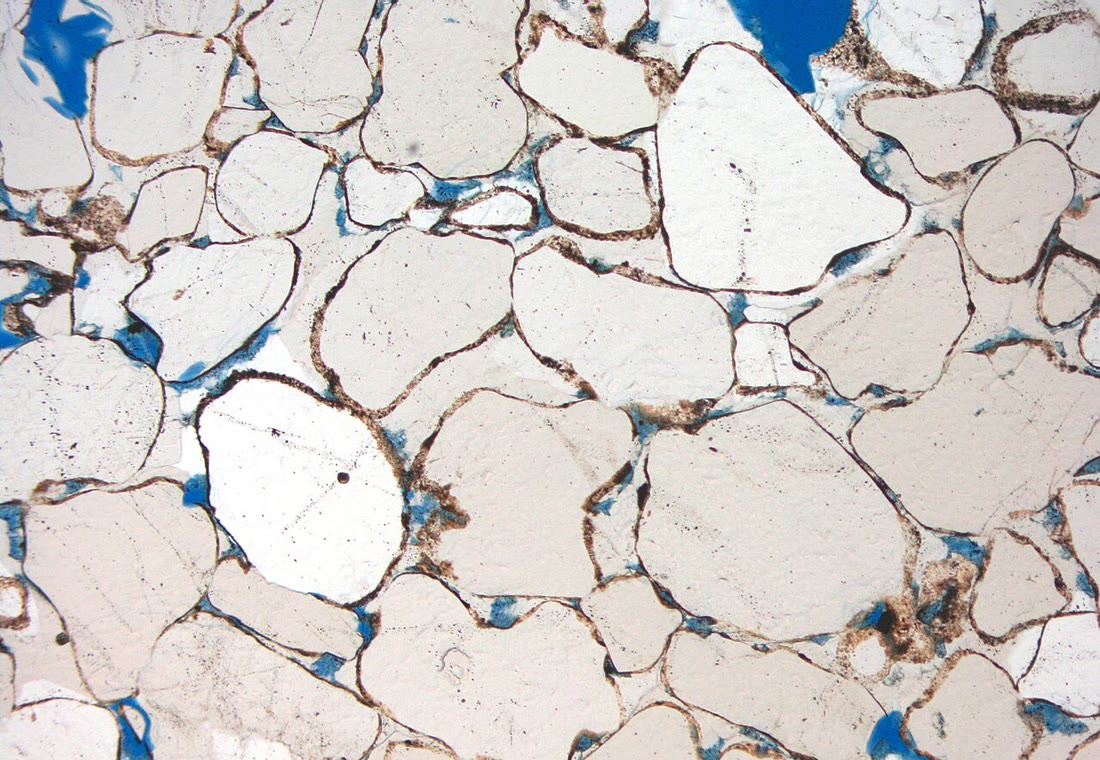
\includegraphics[width=0.62\linewidth]{images/book3/b1-quartz-overgrowths.jpg}

{\small \omterm{def:b1:field-lab-methods-1:thin-section}{Sayatan tipis} batu pasir kuarsa, Batu Pasir Potsdam (Kambrium) di Negara Bagian New York, dalam \omterm{def:b1:field-lab-methods-1:microscope}{cahaya terpolarisasi bidang}. Butiran detrital yang membulat dibatasi tepinya oleh pinggiran gelap debu dan lempung; kuarsa jernih di luar pinggiran adalah \omterm{def:b1:diagenesis-basins:cement}{semen} yang tumbuh pada butiran, secara optik kontinu dengannya, sampai tepi-tepi tambahan yang berdekatan bertemu sepanjang permukaan lurus. Resin biru mengisi sisa pori-pori. (M.~C.~Rygel, CC~BY-SA~4.0, melalui Wikimedia Commons; batang skala pada aslinya telah dipotong.)}
\label{fig:b1:diagenesis-basins:overgrowths}
\end{omfigure}
% ledger: commons:potsdam

Tidak semua perubahan menghancurkan porositas. Air yang tidak jenuh terhadap suatu \omterm{def:b1:rock-forming-minerals:mineral}{mineral} akan melarutkannya: butiran \omterm{def:b1:rock-forming-minerals:groups}{feldspar} dan karbonat, dan \omterm{def:b1:diagenesis-basins:cement}{semen} karbonat yang lebih awal, dapat dibuang dan meninggalkan porositas sekunder, pori-pori berbentuk seperti butiran yang digantikannya. \omterm{def:b1:weathering-clays:clay-mineral}{Mineral lempung} tumbuh di dalam pori-pori pada gilirannya, sebagai lapisan pada butiran atau sebagai kristal yang mengisi pori dan mempersempit jalan di antaranya, sehingga menurunkan permeabilitas. \omterm{def:b1:rock-forming-minerals:mineral}{Mineral} sedimen juga berubah: aragonit cangkang dan \omterm{def:b1:chemical-biogenic-sediments:factory}{pabrik karbonat} kembali menjadi kalsit, yang stabil di permukaan, dan kalsit dalam air yang mengandung magnesium dapat menjadi dolomit.
% ledger: og:diagenesis

Penggantian kalsit oleh dolomit, dolomitisasi, adalah reaksi dengan magnesium dari air,
\[
  \ce{2 CaCO3 + Mg^2+ -> CaMg(CO3)2 + Ca^2+},
\]
dan ia mengubah volume padatan.

\begin{proposition}[Dolomitisasi menciptakan porositas]\label{prop:b1:diagenesis-basins:dolomite}
Jika dua mol kalsit dengan massa jenis $\rho_c$ digantikan oleh satu mol dolomit dengan massa jenis $\rho_d$, volume padatan berkurang sebesar fraksi
\[
  1 - \frac{M_d/\rho_d}{2M_c/\rho_c},
\]
di mana $M_c$ dan $M_d$ adalah massa molar. Dengan $\rho_c = \qty{2.71}{g.cm^{-3}}$ dan $\rho_d = \qty{2.84}{g.cm^{-3}}$ fraksi ini adalah \qty{12.1}{\percent}.
\end{proposition}

\begin{proof}
Volume molar suatu \omterm{def:b1:rock-forming-minerals:mineral}{mineral} adalah massa molarnya dibagi massa jenisnya. Dua mol kalsit menempati $2M_c/\rho_c$ dan satu mol dolomit $M_d/\rho_d$; fraksi yang hilang adalah satu dikurangi rasio keduanya. Dengan $M_c = \qty{100.09}{g.mol^{-1}}$ dan $M_d = \qty{184.40}{g.mol^{-1}}$ kedua volume itu adalah
$2\times\qty{36.93}{cm^3} = \qty{73.86}{cm^3}$ dan \qty{64.93}{cm^3}, dan $1 - 64.93/73.86 = \num{0.121}$.
\end{proof}

Jika volume luar batuan tidak berubah, padatan yang hilang adalah ruang pori yang diperoleh: batu kapur dengan porositas \num{0.10} yang digantikan mol demi mol oleh dolomit memiliki porositas sekitar \num{0.21}. Reaksi ini membutuhkan magnesium dalam jumlah besar, yang dikandung air laut sekitar \qty{1.28}{g} per kilogram; ia lebih mudah terjadi di tempat air asin atau air laut mengalir melalui batuan dalam waktu lama (\cref{exo:b1:diagenesis-basins:12}).
% ledger: hom:calcite, webmineral:others, teos10:reference-composition, teos10:reference-salinity

\omterm{def:b1:diagenesis-basins:diagenesis}{Diagenesis} mengikuti sejarah sedimen. Tepat setelah pengendapan, dekat permukaan, air pori masih air laut, danau atau hujan: sedimen dilubangi, disemen lebih awal di dasar laut atau di tanah, dan aragonit berubah menjadi kalsit. Dengan penguburan dan pemanasan, \omterm{def:b1:diagenesis-basins:compaction}{pemadatan}, pelarutan tekanan dan \omterm{def:b1:diagenesis-basins:cement}{semen} kuarsa mendominasi. Jika cekungan kemudian terangkat dan tererosi, air tawar dari permukaan mengalir kembali ke dalam batuan, dan melarutkan karbonat serta \omterm{def:b1:rock-forming-minerals:groups}{feldspar} lagi. Sebuah \omterm{def:b1:field-lab-methods-1:thin-section}{sayatan tipis} mencatat urutan peristiwa-peristiwa ini: \omterm{def:b1:diagenesis-basins:cement}{semen} yang mengisi pori yang ditinggalkan oleh butiran yang larut lebih muda daripada pelarutannya, dan tepi tambahan yang patah oleh \omterm{def:b1:diagenesis-basins:compaction}{pemadatan} lebih tua daripada \omterm{def:b1:diagenesis-basins:compaction}{pemadatan}.

\section{Cekungan sedimen}\label{sec:b1:diagenesis-basins:basins}

Sedimen setebal kilometer hanya terakumulasi di tempat dasarnya terus turun.

\begin{definition}[Cekungan sedimen]\label{def:b1:diagenesis-basins:basin}
Sebuah \emph{cekungan sedimen}\index{cekungan sedimen} adalah wilayah permukaan Bumi tempat \omterm{def:b1:layered-earth:layers}{kerak} telah turun dalam waktu lama, dari beberapa juta hingga beberapa ratus juta tahun, dan tempat ruang yang tercipta dengan demikian telah terisi sedimen, setebal ratusan meter hingga banyak kilometer.
\end{definition}

\begin{definition}[Penurunan, penurunan tektonik]\label{def:b1:diagenesis-basins:subsidence}
\emph{Penurunan}\index{penurunan} suatu cekungan adalah gerak turun dasarnya, permukaan tempat sedimennya bertumpu, diukur relatif terhadap acuan tetap seperti pusat Bumi. \emph{Penurunan tektonik}\index{penurunan tektonik} adalah bagian yang disebabkan oleh proses-proses yang membentuk cekungan, berbeda dari penurunan tambahan akibat berat sedimen dan air yang mengisinya; ia diukur sebagai penurunan yang akan dialami dasar di bawah air saja.
\end{definition}

Yang membuat dasar turun adalah letak cekungan dalam lempeng (gambar di bawah).

\begin{description}
  \item[Cekungan celah.] \omterm{def:b1:faults-folds-fabrics:fault-types}{Sesar normal} meregangkan \omterm{def:b1:layered-earth:layers}{kerak}, dan blok-blok turun di antaranya (\cref{ch:b1:rifts-ridges-margins}). Cekungan itu sempit dan asimetris, setengah \omterm{def:b1:rifts-ridges-margins:rift}{graben} yang terisi paling cepat di dekat sesar tepinya. Ladang minyak Laut Utara terletak dalam struktur \omterm{def:b1:rifts-ridges-margins:rift}{Graben} Viking dan \omterm{def:b1:rifts-ridges-margins:rift}{Graben} Tengah, terkubur di bawah sedimen yang lebih muda. Ketika peregangan berhenti, \omterm{def:b1:layered-earth:lithosphere}{litosfer} yang menipis dan memanas mendingin, menyusut dan terus turun, perlahan, selama puluhan juta tahun. Laut Utara bagian tengah, yang peregangan besar terakhirnya berakhir pada pertengahan Kapur, kemudian tenggelam sebagai cekungan lebar berbentuk piring, terisi berturut-turut oleh kapur, batu pasir dan, sepanjang sebagian besar Tersier, serpih dan batulumpur; batuan dasarnya, dibebani oleh air saja, akan turun \qtyrange{1100}{1400}{m} di bagian tengahnya.
  \item[Margin pasif.] Di tempat celah menjadi samudra, pendinginan yang sama membuat setiap margin turun setelah pemisahan, dan sebuah baji sedimen yang menebal ke arah samudra terbentuk di atas cekungan celah lama.
  \item[Cekungan depan-pegunungan.] Di depan sabuk \omterm{def:b1:faults-folds-fabrics:fault-types}{sesar dorong}, berat lembaran-lembaran \omterm{def:b1:faults-folds-fabrics:fault-types}{sesar dorong} yang bertumpuk melengkungkan \omterm{def:b1:layered-earth:lithosphere}{litosfer} ke bawah, secara isostatik, menjadi cekungan yang paling dalam di dekat sabuk itu dan terisi oleh puing yang tererosi darinya. Sebagian besar batuan Kapur di Kanada barat diendapkan di cekungan semacam itu di depan Pegunungan Rocky.
  \item[Cekungan intrakratonik.] Di pedalaman benua tua, jauh dari batas lempeng mana pun, wilayah-wilayah lebar berbentuk bulat atau lonjong telah turun perlahan selama waktu yang sangat panjang. Cekungan Paris adalah pusat depresi struktural semacam itu, di antara massif-massif tua Bretagne, Masif Sentral, serta Vosges dan Ardennes.
  \item[Cekungan geser-mendatar.] Di tempat \omterm{def:b1:faults-folds-fabrics:fault-types}{sesar geser-mendatar} menggeser ke samping dalam arah yang menarik dindingnya terpisah --- sebuah tikungan pelepas --- sebuah jajar genjang \omterm{def:b1:layered-earth:layers}{kerak} turun di antara kedua untai sesar: sebuah cekungan tarik-apart, seperti yang ada di kawasan Los Angeles di sepanjang sistem San Andreas.
\end{description}
% ledger: ws:basins, sc80:north-sea, britannica:paris-basin

Mengapa \omterm{def:b1:layered-earth:lithosphere}{litosfer} turun di tiap latar, dengan laju berapa, dan bagaimana cekungan-cekungan itu dibandingkan, menjadi pokok bahasan volume Tahun ke-2; di sini mereka dibedakan menurut letaknya dan bentuk isiannya.

\begin{omfigure}
\begin{tikzpicture}[font=\scriptsize, line join=round]
% (a) rift: a half-graben
\begin{scope}
  \fill[lith granite] (0,0) -- (0,1.6) -- (1.4,1.6) -- (2.2,0.2) -- (5.0,1.0) -- (5.0,0) -- cycle;
  \fill[lith shale] (1.4,1.6) -- (2.2,0.2) -- (5.0,1.0) -- (5.0,1.6) -- cycle;
  \fill[lith sandstone] (1.4,1.6) -- (1.75,0.99) -- (5.0,1.25) -- (5.0,1.6) -- cycle;
  \draw[normal fault, thick] (1.4,1.6) -- (2.3,0.0);
  \draw[black!70] (0,1.6) -- (5.0,1.6);
  \node[anchor=south west] at (0,1.65) {(a) celah: setengah graben};
  \node[fill=white, fill opacity=0.8, text opacity=1, inner sep=1pt] at (3.9,0.3) {batuan dasar};
  \node[fill=white, fill opacity=0.8, text opacity=1, inner sep=1pt] at (0.65,0.8) {dinding bawah};
\end{scope}
% (b) passive margin: a seaward-thickening wedge over thinned crust
\begin{scope}[xshift=6.6cm]
  \fill[lith sea] (2.0,1.6) -- (5.0,1.6) -- (5.0,0.75) -- (3.6,0.95) -- cycle;
  \fill[lith granite] (0,0) -- (0,1.2) -- (2.0,1.0) -- (3.6,0.35) -- (5.0,0.05) -- (5.0,0) -- cycle;
  \fill[lith shale] (0,1.2) -- (2.0,1.0) -- (3.6,0.35) -- (5.0,0.05) -- (5.0,0.75) -- (3.6,0.95) -- (2.0,1.6) -- (0,1.6) -- cycle;
  \draw[black!70] (0,1.6) -- (2.0,1.6) -- (3.6,0.95) -- (5.0,0.75);
  \draw[blue!60!black, thick] (2.0,1.6) -- (5.0,1.6);
  \node[anchor=south west] at (0,1.65) {(b) margin pasif};
  \node[fill=white, fill opacity=0.8, text opacity=1, inner sep=1pt] at (1.0,0.45) {kerak benua yang menipis};
  \node[anchor=north east] at (5.0,1.58) {laut};
\end{scope}
% (c) foreland basin: asymmetric, deepest against the thrust belt
\begin{scope}[yshift=-3.3cm]
  \fill[lith granite] (0,0) -- (0,0.55) -- (5.0,1.35) -- (5.0,0) -- cycle;
  \fill[lith sandstone] (0,0.55) -- (5.0,1.35) -- (5.0,1.6) -- (0,1.6) -- cycle;
  \fill[lith conglomerate] (1.0,1.6) -- (3.6,1.6) -- (1.0,1.0) -- cycle;
  \fill[omLithSchist, draw=black!70] (0,0.95) -- (1.9,1.6) -- (1.3,1.95) -- (0.4,2.25) -- (0,2.3) -- cycle;
  \draw[thrust fault] (0,0.95) -- (1.9,1.6);
  \draw[thrust fault] (0,1.55) -- (1.15,1.95);
  \draw[black!70] (1.9,1.6) -- (5.0,1.6);
  \node[anchor=south west] at (2.0,1.65) {(c) cekungan depan-pegunungan};
  \node[anchor=south west, inner sep=1pt] at (0.25,2.3) {sabuk sesar dorong};
  \node[fill=white, fill opacity=0.8, text opacity=1, inner sep=1pt] at (3.9,0.35) {batuan dasar};
\end{scope}
% (d) intracratonic basin: a broad sag, layers thickening to the centre
\begin{scope}[xshift=6.6cm, yshift=-3.3cm]
  \fill[lith granite] (0,0) -- (0,1.5) .. controls (1.6,1.1) and (2.0,0.3) .. (2.5,0.3) .. controls (3.0,0.3) and (3.4,1.1) .. (5.0,1.5) -- (5.0,0) -- cycle;
  \fill[lith limestone] (0,1.5) .. controls (1.6,1.1) and (2.0,0.3) .. (2.5,0.3) .. controls (3.0,0.3) and (3.4,1.1) .. (5.0,1.5) -- (5.0,1.6) -- (0,1.6) -- cycle;
  \fill[lith shale] (0.6,1.6) .. controls (1.6,1.35) and (2.1,0.85) .. (2.5,0.85) .. controls (2.9,0.85) and (3.4,1.35) .. (4.4,1.6) -- cycle;
  \fill[lith sandstone] (1.3,1.6) .. controls (1.9,1.5) and (2.2,1.3) .. (2.5,1.3) .. controls (2.8,1.3) and (3.1,1.5) .. (3.7,1.6) -- cycle;
  \draw[black!70] (0,1.6) -- (5.0,1.6);
  \node[anchor=south west] at (0,1.65) {(d) cekungan intrakratonik};
  \node[fill=white, fill opacity=0.8, text opacity=1, inner sep=1pt] at (4.2,0.4) {batuan dasar};
\end{scope}
\end{tikzpicture}

{\small Empat jenis \omterm{def:b1:diagenesis-basins:basin}{cekungan sedimen} dalam penampang (skematis, tidak dalam skala; skala vertikal dilebih-lebihkan). (a)~Sebuah celah: isiannya menebal ke arah sesar tepi setengah \omterm{def:b1:rifts-ridges-margins:rift}{graben}. (b)~Margin pasif: sebuah baji sedimen yang menebal ke arah samudra di atas \omterm{def:b1:layered-earth:layers}{kerak} benua yang menipis. (c)~Cekungan depan-pegunungan, paling dalam di dekat sabuk \omterm{def:b1:faults-folds-fabrics:fault-types}{sesar dorong} yang beratnya melengkungkannya ke bawah, dan terisi oleh puingnya, yang paling kasar (konglomerat) di dekat sabuk; sabuk itu menindih tepi cekungannya sendiri. (d)~Cekungan intrakratonik: depresi lebar yang lapisannya menebal ke arah pusat.}
\label{fig:b1:diagenesis-basins:types}
\end{omfigure}

\begin{inthefield}[Bagaimana cekungan diketahui]
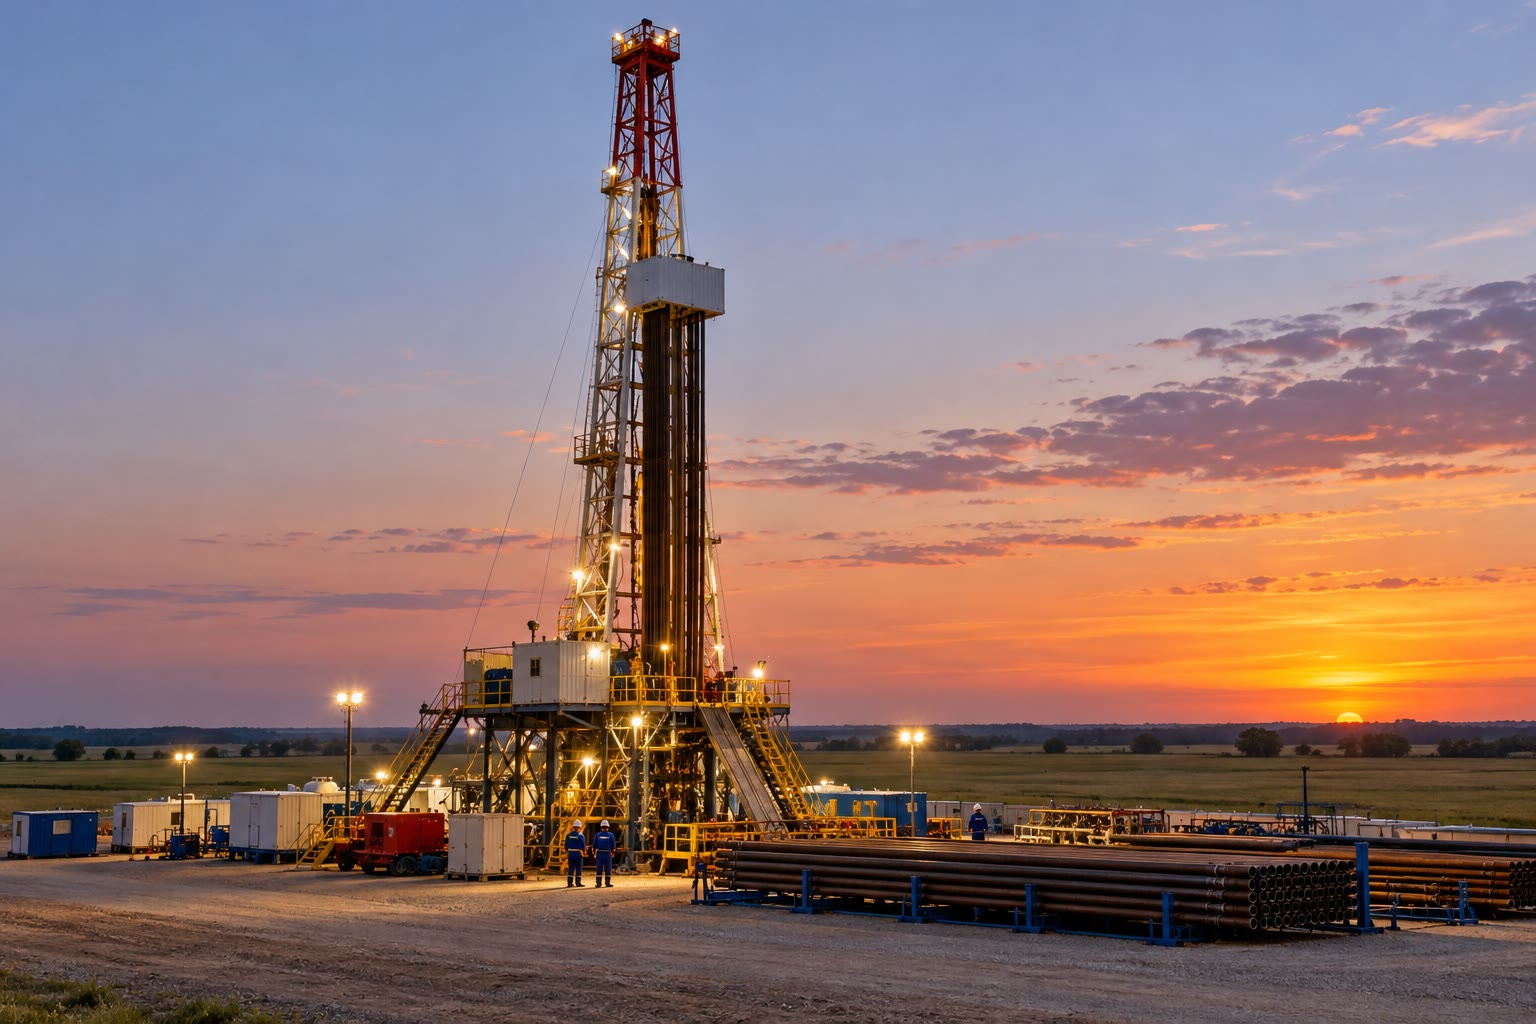
\includegraphics[width=0.3\linewidth]{images/book3/ai/b1-drilling-rig.jpg}\hfill
\begin{minipage}[b]{0.67\linewidth}
Hampir semua yang diketahui tentang isian dalam sebuah cekungan berasal dari pencarian minyak, gas dan air. Survei refleksi seismik mencitrakan lapisan-lapisannya dan sesarnya di atas ribuan kilometer persegi; sumur mencicipinya di satu titik. Sebuah sumur mengembalikan serpihan batuan yang dipotong oleh mata bor, pada interval berupa inti, dan log kontinu sifat fisika batuan di sekitar lubang, dari mana porositas dibaca meter demi meter. Kurva porositas--kedalaman \omterm{prop:b1:diagenesis-basins:athy}{hukum Athy}, dan sejarah \omterm{def:b1:diagenesis-basins:subsidence}{penurunan} cekungan, pertama kali dibangun dari sumur semacam itu.
\end{minipage}

\smallskip
{\small Sebuah rig bor darat pada senja hari, pipa tersusun di rak di latar depan (ilustrasi AI).}
\end{inthefield}
% ledger: sc80:north-sea

\section{Penurunan, akomodasi dan muka laut}\label{sec:b1:diagenesis-basins:accommodation}

Sedimen hanya dapat menumpuk di tempat ada ruang untuknya di bawah tingkat tempat ia akan dipindahkan. Di laut tingkat itu dekat dengan permukaan laut, dan ruangnya adalah soal dua gerak: gerak dasar, dan gerak permukaan laut.

\begin{definition}[Akomodasi]\label{def:b1:diagenesis-basins:accommodation}
\emph{Akomodasi}\index{akomodasi} di suatu titik cekungan adalah ruang yang tersedia bagi sedimen untuk terakumulasi di sana: jarak tegak dari puncak sedimen ke permukaan laut, tingkat dasar pengendapan laut. Akomodasi yang tercipta dalam suatu interval waktu adalah kenaikan jarak dari sebuah datum yang melekat pada batuan dasar ke permukaan laut.
\end{definition}

\begin{definition}[Eustasi, muka laut relatif]\label{def:b1:diagenesis-basins:eustasy}
\emph{Eustasi}\index{eustasi} adalah perubahan tinggi samudra dunia yang diukur relatif terhadap acuan tetap, pusat Bumi, yang disebabkan oleh perubahan volume air di laut atau volume cekungan samudra; ia sama di mana-mana. \emph{Muka laut relatif}\index{muka laut relatif} di suatu tempat adalah tinggi permukaan laut di atas datum yang melekat pada batuan dasar di sana; ia berubah oleh eustasi dan oleh gerak vertikal tanah.
\end{definition}

\begin{proposition}[Anggaran akomodasi]\label{prop:b1:diagenesis-basins:budget}
Dalam suatu interval waktu, misalkan $\Delta E$ adalah kenaikan eustatik muka laut dan $S$ \omterm{def:b1:diagenesis-basins:subsidence}{penurunan} batuan dasar (keduanya positif ke atas bagi laut, ke bawah bagi dasar). \omterm{def:b1:diagenesis-basins:accommodation}{Akomodasi} yang tercipta adalah
\[
  \Delta A = \Delta E + S ,
\]
dan ia dibagi antara ketebalan sedimen yang ditambahkan di atas datum, $\Delta T$, dan pendalaman air, $\Delta W$: $\Delta E + S = \Delta T + \Delta W$.
\end{proposition}

\begin{proof}
Ukur tinggi dari acuan tetap. Misalkan $e$ adalah tinggi permukaan laut, $b$ tinggi datum, $T$ ketebalan sedimen di atas datum, dan $W$ kedalaman air di atas sedimen, sehingga $e = b + T + W$. \omterm{def:b1:diagenesis-basins:eustasy}{Muka laut relatif} adalah $R = e - b = T + W$. Selama interval itu, $\Delta e =
\Delta E$ dan $\Delta b = -S$, sehingga $\Delta R = \Delta E + S$; dan $\Delta R =
\Delta T + \Delta W$.
\end{proof}

Dasar laut yang dipertahankan pada kedalaman tetap ($\Delta W = 0$) terisi tepat secepat \omterm{def:b1:diagenesis-basins:accommodation}{akomodasi} tercipta; yang menjadi dangkal terisi lebih cepat, dan garis pantai bergerak ke laut; yang makin dalam mengalami kekurangan sedimen. $\Delta T$ adalah perubahan ketebalan seluruh tumpukan di atas datum: ia menghitung sedimen baru yang diendapkan, dikurangi penipisan sedimen yang lebih tua di bawahnya ketika mereka memadat, sehingga \omterm{def:b1:diagenesis-basins:compaction}{pemadatan} sendiri menciptakan ruang bagi lebih banyak sedimen (gambar di bawah).

\begin{omfigure}
\begin{tikzpicture}[font=\footnotesize, >=Stealth]
\def\col#1#2#3#4#5{% x, datum, sediment top, sea, label
  \fill[lith granite] (#1,0.2) rectangle ++(1.4,#2-0.2);
  \fill[lith shale] (#1,#2) rectangle ++(1.4,#3-#2);
  \fill[lith sea] (#1,#3) rectangle ++(1.4,#4-#3);
  \draw[black!70] (#1,#2) -- ++(1.4,0);
  \draw[blue!60!black, thick] (#1-0.2,#4) -- ++(1.8,0);
  \node[anchor=north] at (#1+0.7,0.15) {#5};}
\draw[black!60, dash dot] (-0.6,0.9) -- (8.6,0.9) node[anchor=west, align=left] {acuan\\ tetap};
\col{0}{1.5}{3.0}{3.6}{waktu $t_1$}
\col{4.4}{1.0}{3.4}{3.9}{waktu $t_2$}
% eustasy
\draw[<->, omThm] (3.0,0.9) -- (3.0,3.6) node[midway, fill=white, inner sep=1pt] {$e_1$};
\draw[<->, omThm] (7.4,0.9) -- (7.4,3.9) node[midway, fill=white, inner sep=1pt] {$e_2$};
% subsidence of the datum
\draw[dashed, black!60] (1.4,1.5) -- (4.4,1.5);
\draw[->, thick] (4.2,1.5) -- (4.2,1.0) node[midway, anchor=east] {$S$};
% relative sea level
\draw[<->] (-0.35,1.5) -- (-0.35,3.6) node[midway, anchor=east] {$R_1$};
\draw[<->] (6.05,1.0) -- (6.05,3.9) node[midway, anchor=west] {$R_2$};
\node[anchor=west] at (1.5,2.25) {$T_1$};
\node[anchor=west] at (1.5,3.3) {$W_1$};
\node at (5.1,2.2) {$T_2$};
\node at (5.1,3.65) {$W_2$};
\node[anchor=south, align=center, blue!60!black] at (5.1,3.95) {muka laut};
\node[anchor=west, align=left, font=\scriptsize] at (8.6,2.4) {$R = e - b = T + W$\\[2pt] $\Delta R = \Delta E + S$\\ $\phantom{\Delta R} = \Delta T + \Delta W$};
\end{tikzpicture}

{\small \omterm{def:b1:diagenesis-basins:accommodation}{Akomodasi} di satu tempat pada dua waktu (skematis). Antara $t_1$ dan $t_2$ muka laut naik sebesar $\Delta E = e_2 - e_1$ di atas acuan tetap dan batuan dasar turun sebesar $S$: \omterm{def:b1:diagenesis-basins:eustasy}{muka laut relatif} $R$ tumbuh sebesar $\Delta E + S$, \omterm{def:b1:diagenesis-basins:accommodation}{akomodasi} yang tercipta, yang dibagi antara lebih banyak sedimen ($T_2 > T_1$) dan perubahan kedalaman air (di sini pendangkalan kecil, $W_2 < W_1$).}
\label{fig:b1:diagenesis-basins:accommodation}
\end{omfigure}

Suatu cekungan tidak turun oleh \omterm{def:b1:diagenesis-basins:subsidence}{penurunan tektoniknya} saja: sedimen yang mengisinya adalah beban, dan \omterm{def:b1:layered-earth:lithosphere}{litosfer} turun lebih jauh di bawahnya.

\begin{proposition}[Beban sedimen memperkuat penurunan]\label{prop:b1:diagenesis-basins:loading}
Dalam \omterm{def:b1:isostasy-gravity:isostasy}{isostasi} lokal (Airy) di atas \omterm{def:b1:layered-earth:layers}{mantel} bermassa jenis $\rho_m$, sebuah cekungan yang batuan dasarnya, dibebani oleh air bermassa jenis $\rho_w$ saja, akan berada pada kedalaman $Y$ di bawah permukaan laut, ketika diisi sampai permukaan laut dengan sedimen bermassa jenis rerata $\rho_s$, memiliki ketebalan
\[
  h = Y\,\frac{\rho_m - \rho_w}{\rho_m - \rho_s}
\]
sedimen. Di darat, diisi sampai ke tingkat sekitarnya dengan udara di atasnya, faktornya adalah $\rho_m/(\rho_m - \rho_s)$.
\end{proposition}

\begin{proof}
Bandingkan dua kolom dengan \omterm{def:b1:layered-earth:lithosphere}{litosfer} yang sama, bermassa $M$ per satuan luas dan tebal $L$, hingga \omterm{def:b1:isostasy-gravity:isostasy}{kedalaman kompensasi} $z_c$ di bawah keduanya. Kolom yang dibebani air memuat $\rho_w Y + M + \rho_m(z_c - Y - L)$; yang terisi sedimen $\rho_s h + M + \rho_m(z_c - h - L)$. Dengan \cref{prop:b1:isostasy-gravity:equal-mass} kedua massa itu sama, sehingga $\rho_w Y - \rho_m Y = \rho_s h - \rho_m h$, yakni $h(\rho_m - \rho_s) =
Y(\rho_m - \rho_w)$. Dengan udara menggantikan air, $\rho_w$ diganti nol.
\end{proof}

Dengan $\rho_m = \qty{3300}{kg.m^{-3}}$, $\rho_w = \qty{1030}{kg.m^{-3}}$ dan sedimen dengan massa jenis rerata \qty{2300}{kg.m^{-3}}, faktornya adalah $2270/1000 = \num{2.27}$: sebuah cekungan yang \omterm{def:b1:diagenesis-basins:subsidence}{penurunan tektoniknya} akan menyediakan ruang bagi \qty{1}{km} air menampung \qty{2.27}{km} sedimen. Di darat faktornya adalah $3300/1000 = \num{3.3}$. Massa jenis isian tidak konstan: ia tumbuh ketika sedimen memadat, dan faktornya ikut tumbuh, sehingga mengubah ketebalan sedimen menjadi \omterm{def:b1:diagenesis-basins:subsidence}{penurunan tektonik} membutuhkan \omterm{def:b1:diagenesis-basins:compaction}{dekompaksi} setiap lapisan, langkah waktu demi langkah waktu. Prosedur itu, penelusuran mundur (backstripping), termasuk dalam volume Tahun ke-2.

Muka laut sendiri jauh dari tetap. Pada Maksimum Glasial Terakhir, lembaran es menutupi sebagian besar Amerika Utara dan Eropa utara, dan air yang terkunci di dalamnya telah diambil dari samudra. Setelah dikoreksi untuk tanggapan Bumi padat terhadap beban es dan air yang berubah, pengamatan terhadap garis pantai purba memberikan muka laut yang turun dengan cepat sekitar \qty{40}{m} sekitar \num{30000} tahun yang lalu dan kemudian perlahan, hingga \qty{134}{m} di bawah hari ini, dari \qtyrange{29}{21}{\ka}; lembaran es darat kemudian menahan sekitar \qty{52e6}{km^3} lebih banyak daripada hari ini. Angka \qty{125}{m} yang sering dikutip lebih kecil karena biasanya tidak dikoreksi untuk efek isostatik ini. Deglasiasi terutama terjadi antara sekitar \qty{16.5}{\ka} dan \qty{8.2}{\ka}, rata-rata \qty{12}{m} per seribu tahun, dan pada \qty{40}{mm} setahun atau lebih antara \qty{14.5}{\ka} dan \qty{14.0}{\ka}.
% ledger: lambeck:lgm, lambeck:deglaciation

Muka laut rendah yang lebih tua dibaca dari isotop oksigen foraminifera dalam inti dasar laut dalam, yang mencatat volume es di darat. Menumpuk tujuh rekonstruksi semacam itu selama \num{430000} tahun terakhir, dan lima selama \num{800000} terakhir, merata-ratakan kesalahan masing-masing; diskalakan ke Holosen dan ke muka laut rendah glasial terakhir, tumpukan itu membawa ketidakpastian \qtyrange{9}{12}{m} (gambar di bawah). Ia menunjukkan siklus glasial sebagai gigi gergaji: penurunan muka laut yang lambat, masing-masing diakhiri oleh kenaikan yang cepat --- lima kali dalam \num{800000} tahun terakhir sebuah kenaikan lebih dari \qty{100}{m} dalam kurang dari \num{20000} tahun. \omterm{def:b1:diagenesis-basins:eustasy}{Eustasi} pada skala ini menggerakkan garis pantai maju-mundur melintasi paparan benua.
% ledger: spratt:stack, data:b3-sealevel-stack

\begin{omfigure}
\begin{tikzpicture}[font=\footnotesize]
\begin{axis}[width=16cm, height=4.8cm, xmin=0, xmax=800, ymin=-150, ymax=40,
    x dir=reverse, xlabel={umur (ribuan tahun sebelum sekarang)}, xlabel style={yshift=2pt},
    ylabel={muka laut (m)}, ytick={-150,-100,-50,0},
    title={(a) \num{800000} tahun terakhir (lima rekaman)}, title style={font=\footnotesize},
    axis on top]
  \addplot[draw=none, name path=hi] table[x=age, y=hi] {figdata/out/bachelor-1-sea_level-long.dat};
  \addplot[draw=none, name path=lo] table[x=age, y=lo] {figdata/out/bachelor-1-sea_level-long.dat};
  \addplot[omThm!25] fill between[of=hi and lo];
  \addplot[thin, omThm] table[x=age, y=sl] {figdata/out/bachelor-1-sea_level-long.dat};
  \draw[black!50, densely dotted] (axis cs:0,0) -- (axis cs:800,0);
\end{axis}
\end{tikzpicture}

\medskip
\begin{tikzpicture}[font=\footnotesize]
\begin{axis}[width=16cm, height=4.8cm,
    xmin=0, xmax=140, ymin=-160, ymax=40, x dir=reverse,
    xlabel={umur (ribuan tahun sebelum sekarang)}, ylabel={muka laut (m)},
    ytick={-150,-100,-50,0},
    title={(b) \num{140000} tahun terakhir (tujuh rekaman)}, title style={font=\footnotesize},
    axis on top]
  \addplot[draw=none, name path=hi] table[x=age, y=hi] {figdata/out/bachelor-1-sea_level-short.dat};
  \addplot[draw=none, name path=lo] table[x=age, y=lo] {figdata/out/bachelor-1-sea_level-short.dat};
  \addplot[omThm!25] fill between[of=hi and lo];
  \addplot[thick, omThm] table[x=age, y=sl] {figdata/out/bachelor-1-sea_level-short.dat};
  \draw[black!50, densely dotted] (axis cs:0,0) -- (axis cs:140,0);
  \addplot[only marks, mark=*, mark size=1.6pt, black] coordinates {(21,-134)};
  \draw[black!60, thin] (axis cs:21,-131) -- (axis cs:21,-46);
  \node[anchor=south, font=\scriptsize, fill=white, inner sep=1pt] at (axis cs:36,-46) {\qty{-134}{m} pada \qty{21}{\ka} dari garis pantai (Lambeck dkk.\ 2014)};
\end{axis}
\end{tikzpicture}

{\small Muka laut global relatif terhadap hari ini dari tumpukan Spratt dan Lisiecki (2016): komponen utama pertama dari lima rekonstruksi dari inti dasar laut selama \num{800000} tahun (a) dan dari tujuh selama \num{140000} tahun terakhir (b), dengan pita satu simpangan baku. Nilai terendah tumpukan, \qty{-130}{m} pada \qty{24}{\ka}, terletak di dalam pita itu dari \qty{-134}{m} yang ditemukan dari garis pantai purba (titik); interglasial terakhir berdiri sekitar \qty{3}{m} di atas hari ini pada \qty{121}{\ka}. Data: Layanan Data Dunia NOAA NCEI untuk Paleoklimatologi.}
\label{fig:b1:diagenesis-basins:sea-level}
\end{omfigure}
% computed in figdata/bachelor-1/sea_level.py; ledger: data:b3-sealevel-stack, spratt:stack, lambeck:lgm

Dalam kehidupan sebuah cekungan, ayunan seperti itu singkat. Penurunan glasial lebih dari \qty{100}{m} dalam beberapa puluh ribu tahun cepat dan besar dibandingkan dengan \omterm{def:b1:diagenesis-basins:subsidence}{penurunan tektonik}, yang menjumlah menjadi satu kilometer atau lebih hanya selama puluhan juta tahun; tetapi ayunan glasial tetap dalam kisaran sekitar \qty{150}{m}, sehingga dalam isian tebal sebuah cekungan \omterm{def:b1:diagenesis-basins:subsidence}{penurunan} menyediakan sebagian besar ruang, dan \omterm{def:b1:diagenesis-basins:eustasy}{eustasi} menetapkan irama lapisannya.
% ledger: data:b3-sealevel-stack, sc80:north-sea

\section{Latihan}

\begin{exercise}[$\star$]\label{exo:b1:diagenesis-basins:1}
Dengan parameter \cref{tab:b1:diagenesis-basins:athy}, hitunglah porositas batu pasir dan serpih pada \qty{2000}{m}. Pada kedalaman berapakah porositas masing-masing telah turun menjadi setengah dari nilai permukaannya?
% ledger: pybacktrack:compaction
\end{exercise}

\begin{exercise}[$\star$]\label{exo:b1:diagenesis-basins:2}
Selama suatu interval waktu, muka laut naik \qty{30}{m} secara eustatik, batuan dasar sebuah paparan turun \qty{50}{m}, dan \qty{60}{m} sedimen ditambahkan di atas datum pada batuan dasar. Dengan \cref{prop:b1:diagenesis-basins:budget}, hitunglah \omterm{def:b1:diagenesis-basins:accommodation}{akomodasi} yang tercipta dan perubahan kedalaman air. Apakah paparan itu menjadi lebih dalam atau lebih dangkal?
\end{exercise}

\begin{exercise}[$\star$]\label{exo:b1:diagenesis-basins:3}
\omterm{def:b1:diagenesis-basins:subsidence}{Penurunan tektonik} sebuah cekungan akan menyediakan ruang bagi \qty{1.0}{km} air. Dengan $\rho_m = \qty{3300}{kg.m^{-3}}$ dan $\rho_w = \qty{1030}{kg.m^{-3}}$, setebal apakah sedimen yang mengisinya sampai ke permukaan laut jika massa jenis rerata-nya \qty{2300}{kg.m^{-3}}? \qty{2500}{kg.m^{-3}}? Mengapa isian yang lebih padat menghasilkan isian yang lebih tebal?
\end{exercise}

\begin{exercise}[$\star$]\label{exo:b1:diagenesis-basins:4}
Kalsit memiliki massa molar \qty{100.09}{g.mol^{-1}} dan massa jenis \qty{2.71}{g.cm^{-3}}; dolomit \qty{184.40}{g.mol^{-1}} dan \qty{2.84}{g.cm^{-3}}. (a)~Hitunglah volume molar masing-masing. (b)~Dengan fraksi berapakah volume padatan berubah ketika dua mol kalsit menjadi satu mol dolomit? (c)~Sebuah batu kapur dengan porositas \num{0.10} didolomitisasi mol demi mol tanpa perubahan volume luarnya. Berapakah porositas barunya?
% ledger: hom:calcite, webmineral:others
\end{exercise}

\begin{exercise}[$\star\star$]\label{exo:b1:diagenesis-basins:5}
Sebuah serpih menempati \qty{1000}{m} teratas sebuah cekungan. (a)~Hitunglah ketebalan padatnya dan porositas rerata-nya. (b)~Ia dikubur sampai puncaknya berada di \qty{2000}{m}. Dengan \cref{met:b1:diagenesis-basins:decompaction} dengan puncak dipindahkan ke bawah, bukan ke atas, carilah ketebalan barunya dan porositas rerata-nya. (c)~Berapa banyak air yang telah diperas keluar oleh setiap meter persegi serpih itu?
% ledger: pybacktrack:compaction
\end{exercise}

\begin{exercise}[$\star\star$]\label{exo:b1:diagenesis-basins:6}
Sebuah batu pasir terletak antara \qty{2500}{m} dan \qty{2800}{m}. (a)~Hitunglah ketebalan padatnya. (b)~Dekompaksikan ke permukaan dengan \cref{met:b1:diagenesis-basins:decompaction}, tuliskan setiap langkah Newton mulai dari $b_0 = \qty{300}{m}$. (c)~Dengan faktor berapakah penguburan telah menipiskannya?
% ledger: pybacktrack:compaction
\end{exercise}

\begin{exercise}[$\star\star$]\label{exo:b1:diagenesis-basins:7}
Pada Maksimum Glasial Terakhir, es darat menahan sekitar \qty{52e6}{km^3} lebih banyak daripada hari ini. Ambil massa jenis es \qty{916.7}{kg.m^{-3}}, massa jenis air lelehan \qty{1000}{kg.m^{-3}}, dan luas samudra hari ini \qty{361.84e6}{km^2}. (a)~Penurunan muka laut apa yang diwakili es ini? (b)~Bandingkan dengan \qty{134}{m} yang ditemukan dari garis pantai purba. (c)~Berapa luas samudra yang akan memberi tepat \qty{134}{m}, dan mengapa samudra glasial lebih kecil?
% ledger: lambeck:lgm, iapws:ice-density, charette:ocean-volume
\end{exercise}

\begin{exercise}[$\star\star$]\label{exo:b1:diagenesis-basins:8}
Tumpukan muka laut memberikan \qty{-98.1}{m} pada \qty{16}{\ka} dan \qty{-9.1}{m} pada \qty{8}{\ka}. (a)~Hitunglah laju kenaikan rerata, dalam meter per seribu tahun, dan bandingkan dengan \qty{12}{m} per seribu tahun yang ditemukan dari garis pantai purba untuk deglasiasi utama. (b)~Antara \qty{14.5}{\ka} dan \qty{14.0}{\ka} muka laut naik \qty{40}{mm} setahun atau lebih. Berapa kali lipat rerata itu, dan berapa naik muka laut dalam lima ratus tahun itu?
% ledger: data:b3-sealevel-stack, lambeck:deglaciation
\end{exercise}

\begin{exercise}[$\star\star$]\label{exo:b1:diagenesis-basins:9}
Sebuah paparan terletak di bawah \qty{20}{m} air. Batuan dasarnya turun \qty{50}{m} per juta tahun. (a)~Selama dua juta tahun muka laut turun \qty{40}{m} secara eustatik sementara kedalaman air tetap sama. Berapa \omterm{def:b1:diagenesis-basins:accommodation}{akomodasi} yang tercipta, dan berapa sedimen yang ditambahkan? (b)~Muka laut kemudian turun \qty{120}{m} dalam \num{20000} tahun, pada awal glasiasi, dan tidak ada sedimen yang ditambahkan. Seberapa tinggi di atas muka laut dasar laut bekas itu berdiri pada akhirnya?
\end{exercise}

\begin{exercise}[$\star\star\star$]\label{exo:b1:diagenesis-basins:10}
(a)~Tunjukkan bahwa sebuah lapisan setebal $h$ pada kedalaman $z$, tipis dibandingkan dengan
panjang peluruhan $\lambda$, memiliki ketebalan $h_0 \approx h\,(1 - \varphi(z))/(1 -
\varphi_0)$ ketika dipulihkan ke permukaan. (b)~Terapkan pada \qty{10}{m} serpih di \qty{3000}{m}, dan bandingkan dengan \omterm{def:b1:diagenesis-basins:compaction}{dekompaksi} eksak, \qty{23.1}{m}. (c)~Mengapa pendekatan itu sedikit terlalu besar?
% ledger: pybacktrack:compaction
\end{exercise}

\begin{exercise}[$\star\star\star$]\label{exo:b1:diagenesis-basins:11}
Sebuah cekungan diisi sampai permukaan laut oleh \qty{3000}{m} serpih, dipadatkan oleh \omterm{prop:b1:diagenesis-basins:athy}{hukum Athy}, dengan porinya penuh air bermassa jenis \qty{1030}{kg.m^{-3}}. (a)~Hitunglah porositas rerata dan massa jenis rerata isian. (b)~Dengan
\cref{prop:b1:diagenesis-basins:loading} dan $\rho_m =
\qty{3300}{kg.m^{-3}}$, hitunglah faktor pembebanan dan \omterm{def:b1:diagenesis-basins:subsidence}{penurunan} yang diwakili isian oleh air-beban. (c)~Mengapa mengambil massa jenis butiran, \qty{2700}{kg.m^{-3}}, akan memberi faktor yang jauh lebih besar, dan mengapa itu keliru?
% ledger: pybacktrack:compaction
\end{exercise}

\begin{exercise}[$\star\star\star$]\label{exo:b1:diagenesis-basins:12}
Satu meter kubik batu kapur dengan porositas \num{0.10} akan didolomitisasi seluruhnya, mol demi mol. Air laut mengandung \qty{35.165}{g} garam per kilogram, dengan fraksi massa \num{0.0365} adalah magnesium (\qty{24.305}{g.mol^{-1}}). (a)~Berapa mol kalsit yang dikandung kubus itu (volume molar dari
\cref{exo:b1:diagenesis-basins:4})? (b)~Berapa mol magnesium yang dibutuhkan reaksi itu? (c)~Berapa massa dan volume air laut (\qty{1030}{kg.m^{-3}}) yang harus mengalir melalui kubus jika ia memberikan seluruh magnesiumnya? (d)~Apa yang dikatakan jawabannya tentang di mana dolomit terbentuk?
% ledger: teos10:reference-composition, teos10:reference-salinity, hom:calcite
\end{exercise}

\section{Masalah: mendekompaksi isian sebuah cekungan}

\begin{problem}[{Soal akhir pekan --- seberapa tebal sedimen sebuah sumur ketika diendapkan, dan bagaimana ruang baginya dibuat}]
\label{pb:b1:diagenesis-basins:1}
% values: calc/ch23.py; the well, its units, ages and the eustatic changes are invented
Sebuah sumur yang dibor di dataran pantai, di permukaan laut, menembus tiga satuan sebelum mencapai batuan dasar di \qty{3200}{m}:
\begin{center}
\begin{tabular}{llll}
\hline
unit & litologi & kedalaman hari ini (m) & waktu pengendapan \\
\hline
1 & batu pasir & 0--800     & \qtyrange{15}{0}{\Ma} \\
2 & serpih     & 800--2600  & \qtyrange{55}{15}{\Ma} \\
3 & kapur     & 2600--3200 & \qtyrange{75}{55}{\Ma} \\
\hline
\end{tabular}
\end{center}
Ambil parameter \cref{tab:b1:diagenesis-basins:athy}, air pori bermassa jenis \qty{1030}{kg.m^{-3}}, $g = \qty{9.81}{m.s^{-2}}$, dan anggap setiap satuan dipadatkan oleh \omterm{prop:b1:diagenesis-basins:athy}{hukum Athy}, dengan airnya bebas keluar, sepanjang sejarahnya. Mikrofosil menunjukkan bahwa airnya dangkal, dan berkedalaman sama, pada awal dan akhir setiap interval.

\medskip
\noindent\textbf{Bagian I --- Kolom hari ini.}
\begin{enumerate}
  \item Hitunglah porositas di puncak dan di dasar setiap satuan.
  \item Hitunglah porositas rerata setiap satuan.
  \item Berapa banyak air yang dikandung setiap satuan di bawah satu meter persegi?
  \item Hitunglah massa jenis curah setiap satuan, jenuh air, dan massa jenis rerata seluruh kolom.
  \item Hitunglah \omterm{def:b1:stress-strain-rheology:lithostatic}{tekanan litostatik} dan hidrostatik di dasar kolom, dan \omterm{def:b1:stress-strain-rheology:lithostatic}{tegangan efektif} di sana.
  \item Pada kedalaman berapakah porositas batu pasir dan serpih sama? Mana yang lebih berpori di bawahnya?
\end{enumerate}

\noindent\textbf{Bagian II --- Butirannya.}
\begin{enumerate}[resume]
  \item Hitunglah ketebalan padat setiap satuan.
  \item Berapakah ketebalan padat seluruh kolom, dan fraksi apa dari kolom hari ini yang berupa air?
  \item Hitunglah, untuk setiap satuan, laju akumulasi butiran, dalam meter padatan per juta tahun.
  \item Satuan mana yang memiliki pasokan butiran tercepat? Yang paling lambat?
\end{enumerate}

\noindent\textbf{Bagian III --- Satuan-satuan seperti saat diendapkan.}
\begin{enumerate}[resume]
  \item Seberapa tebal batu pasir ketika diendapkan? Mengapa tidak diperlukan perhitungan?
  \item Dekompaksikan serpih ke permukaan: seberapa tebal ia pada \qty{15}{\Ma}, ketika pengendapannya baru saja berakhir?
  \item Dekompaksikan kapur ke permukaan: seberapa tebal ia pada \qty{55}{\Ma}?
  \item Seberapa tebal kapur pada \qty{15}{\Ma}, terkubur di bawah serpih dari pertanyaan sebelumnya?
  \item Berapakah ketebalan seluruh kolom di atas batuan dasar pada \qty{55}{\Ma} dan pada \qty{15}{\Ma}?
  \item Hitunglah laju sedimentasi setiap satuan dari ketebalannya hari ini, dan dari ketebalannya saat diendapkan. Mana yang bermakna?
  \item Dengan fraksi berapakah serpih telah menipis sejak \qty{15}{\Ma}?
\end{enumerate}

\noindent\textbf{Bagian IV --- Menciptakan ruang.}
\begin{enumerate}[resume]
  \item Ambil puncak batuan dasar sebagai datum. Dengan \cref{prop:b1:diagenesis-basins:budget}, hitunglah \omterm{def:b1:diagenesis-basins:accommodation}{akomodasi} yang tercipta dari \qtyrange{75}{55}{\Ma}, dari \qtyrange{55}{15}{\Ma} dan dari \qty{15}{\Ma} hingga hari ini.
  \item Sebuah kurva eustatik untuk wilayah itu memberi muka laut \qty{60}{m} lebih tinggi pada \qty{55}{\Ma} daripada pada \qty{15}{\Ma}, dan \qty{30}{m} lebih tinggi pada \qty{15}{\Ma} daripada hari ini (nilai asumsi). Hitunglah \omterm{def:b1:diagenesis-basins:subsidence}{penurunan} batuan dasar pada dua interval terakhir.
  \item Hitunglah laju \omterm{def:b1:diagenesis-basins:subsidence}{penurunan} rerata di setiap interval, dalam meter per juta tahun.
  \item Berapa bagian \omterm{def:b1:diagenesis-basins:subsidence}{penurunan} yang harus diisi oleh \omterm{def:b1:diagenesis-basins:eustasy}{eustasi} di setiap interval? Apakah \omterm{def:b1:diagenesis-basins:eustasy}{eustasi} membantu atau menghambat pengisian cekungan?
  \item Dari \omterm{def:b1:diagenesis-basins:accommodation}{akomodasi} yang terisi sejak \qty{15}{\Ma}, berapa banyak yang dibuat oleh \omterm{def:b1:diagenesis-basins:compaction}{pemadatan} serpih dan kapur di bawahnya?
  \item Mengapa \omterm{def:b1:diagenesis-basins:subsidence}{penurunan} batuan dasar tidak dapat dibaca dari ketebalan kolom hari ini?
  \item Berapakah ketebalan satuan serpih ketika diendapkan?
\end{enumerate}
\end{problem}
